\section{数値不変量、局所模型の範囲、具体例}\label{sec:examples}

\subsection{coreとEuler数}
一般位置の$m\ge4$直線の補集合$W_m\subset\PP^2$について、compact supports による inclusion-exclusion は
\[
\chi_c(W_m)=3-2m+\binom m2=\binom{m-2}{2}
\]
を与える。
一本を無限遠直線に取れば，$W_m$ は $\CC^2$ 内の一般位置の $m-1$ 本の affine lines の補集合である．
Hattoriの定理\cite{Hattori,PapadimaSuciu}によれば
\[
W_m\simeq(T^{m-1})^{(2)},\qquad
\pi_1(W_m)=\ZZ^{m-1},\qquad
b_1=m-1,\quad b_2=\binom{m-1}{2},
\]
ここで右辺は積CW構造の2次骨格である。
従って Betti 数は有限であり，実四次元の Poincar\'e duality から
$\chi(W_m)=\chi_c(W_m)$ である．
coreはこの補集合のhomotopy typeを持つ。
以下ではこの数値を，構成した写像の全 fiber に沿って確認する．

\begin{proposition}[Fiber Euler 関数の有限支持]
\label{inv:euler-pushforward}
定理\ref{main:global}又は定理\ref{ke:actual-global-fibration}の
全平面構成の $\pi:X_d\to B_d(T)$ を取る．
Core values を $v_1,\ldots,v_d$，相異なる nodal values を
$b_1,\ldots,b_N$ とする．このとき $N=d\binom d2$ であり，
\begin{equation}\label{inv:eq:euler-pushforward}
 (\pi_*\mathbf1)(b):=\chi\bigl(\pi^{-1}(b)\bigr)
 =\sum_{\nu=1}^{N}\mathbf1_{\{b_\nu\}}(b)
  +\binom{d-3}{2}\sum_{i=1}^d\mathbf1_{\{v_i\}}(b).
\end{equation}
ここで開集合の加法的計算には有理定数層の compact-support cohomology の
$\chi_c$ を用い，compact fibers 上ではこれを $\chi$ と書く．
基底を有限個の局所自明な層に分けて Euler 積分できるため，
\begin{equation}\label{inv:euler}
\chi(X_d)=d\binom{d-3}{2}+d\binom d2=d(d^2-4d+6).
\end{equation}
\end{proposition}
\begin{proof}
各二重線上で次数 $d$ の切断は相異なる単純零点を $d$ 個持つ．
一般の構成では各零点に一つの nodal surgery を置き，
actual KE 構成では各 source が一重 pinched torus を与える．
Source は相異なる regular leaves 上に置かれ，
全 fiber の移送と補題\ref{glue:closed-whole-fiber-quotient}は
異なる fibers を同一視しない．従って $N=d\binom d2$ である．

Regular $T^2$ と branch $S^1\times\figeight$ の Euler 数は零である．
一重 pinched torus は $T^2$ の非分離 circle を一点に潰した空間なので，
Euler 数は $\chi(T^2)-\chi(S^1)+1=1$ である．
各 core は $m=d-1$ の直線補集合の有限型 skeleton である．
定理\ref{snc:main}及び補題\ref{ke:positive-residue-finite-type}で，
全 critical values より高い compact regular sublevel $K$ を取り，
index $k$ の critical points の個数を $c_k$ とする．
Critical set は compact 内にあり，Morse 非退化性により $c_k$ は有限である．
補題\ref{ke:compact-relative-morse-smale}の閉 filtration の各差は
$c_k$ 個の stable cells $\mathbb R^k$ の非交和なので，
compact supports の加法性と $K$ の Morse handle 分解から
\[
 \chi_c(\Sigma)=\sum_{k=0}^2(-1)^k c_k
 =\chi(K)=\chi(W_{d-1})=\binom{d-3}{2}.
\]
ここで $K$ より外には critical points がなく，proper exhaustion に沿って
$W_{d-1}$ を $K$ へ deformation retract できる．
この計算に skeleton の Whitney 性は必要ない．
以上が\eqref{inv:eq:euler-pushforward}を与える．

Euler 積分の適用範囲を確認する．Core points，node points，開 branch edges，
および残りの regular two-dimensional regions で基底を有限に層化する．
Regular locus では proper smooth submersion の局所自明性，
branch locus では normal circle と full saddle leaf の product model がある．
Actual 構成の相対葉族補間も全 saddle leaves を同定するので，この局所自明性を保つ．
点層以外を有限個の contractible open cells にさらに分ければ，
各 cell 上の逆像は fiber との積となる．
有限閉 filtration の加法性と積の公式により
\[
 \chi(X_d)=\sum_{S}\chi_c(S)\chi\bigl(\pi^{-1}(b_S)\bigr)
          =\int_{B_d(T)}\pi_*\mathbf1\,d\chi_c .
\]
Regular と branch の項は零，node と core は点層なので，
\eqref{inv:euler}が従う．全写像の subanalytic 性を仮定するのではなく，
構成中の上記の有限層化と局所 product を使っている．
\end{proof}

\begin{corollary}[Cubical 比較写像の fiber Euler 数]
\label{inv:cubical-fiber-euler}
$f=p_T\pi$ に対し，各 $w\in\mathcal C_d$ について
\[
 \chi\bigl(f^{-1}(w)\bigr)
 =\#\{\nu:p_T(b_\nu)=w\}
  +\binom{d-3}{2}\#\{i:p_T(v_i)=w\}.
\]
複数の nodal values が同じ $w$ に写る場合は，その個数を重複度として数える．
これらの fibers は系\ref{topo:cubical-composite-connected}により連結である．
\end{corollary}
\begin{proof}
$p_T^{-1}(w)$ は一点又は有限内部木である．
後者を nodal values と木の頂点で細分すると，
前命題と同じ有限層化の $\pi$ の制限を得る．
Compact な全逆像に対して $\chi_c$ の加法性と積性を用いれば，
regular と branch の項は零で，上式となる．
これは内部木上の全 fiber 合併の計算であり，
その合併の各 smooth part が Lagrangian であるとは主張しない．
\end{proof}

他方、adjunctionと$c(TX_d)=(1+H)^4/(1+dH)$より
\[
K_{X_d}=(d-4)H,\qquad K_{X_d}^2=d(d-4)^2,\qquad
c_2(X_d)=d(d^2-4d+6).
\]
また$p_g=\binom{d-1}{3}$、$q=0$である。
中心成分でも
\[
K_{D_i}+\partial D_i=(d-4)H_i
\]
なのでlog-canonical squaresの和は$d(d-4)^2$となる。
これらは構成の整合性を確認する計算である。
数値不変量が一致することだけから、抽象的なgluingの結果を$X_d$と同定したのではない。

\begin{center}
\begin{tabular}{@{}rrrrrr@{}}
\toprule
$d$ & core一つの$\chi$ & node総数 & $\chi(X_d)$ & $K_{X_d}^2$ & $b_2(B_d)$\\
\midrule
5&1&50&55&5&4\\
6&3&90&108&24&10\\
7&6&147&189&63&20\\
8&10&224&304&128&35\\
9&15&324&459&225&56\\
\bottomrule
\end{tabular}
\end{center}

\subsection{nodal monodromy}\label{inv:nodal-monodromy}
節点の局所機構は、annulus上のconic model
\[
xy=t(z-z_0),\qquad z_0\ne0,
\qquad \left(\frac{|x|^2-|y|^2}{2},\frac{|z|^2}{2}\right)
\]
で見ることができる。
critical pointで$z=z_0+xy/t$を代入すると第二成分の二次部分は
$\operatorname{Re}(\overline{z_0}xy/t)$であり、第一成分とともにfocus--focus pairをなす。
annular circle全体を含めれば、その特異fiberはcompactなpinched torusになる。
定理\ref{main:global}の相対SNC構成では、このmodelの全体をactual collarへ同定する代わりに、局所nodal blow-upとcompact transportを用いる。

line-bundle framingsの下で$xy=t\,s(z)$と書き、regular leaf $\gamma$に沿う$s$のwindingを$k$とする。
両側のangular identificationsの線形部分は
\[
A_k=\begin{pmatrix}-1&k\\0&1\end{pmatrix}.
\]
単純零点を一個横切ると$k$は1だけ増えるので、向きを整えたbasisでは
\[
A_{k+1}A_k^{-1}=\begin{pmatrix}1&1\\0&1\end{pmatrix}.
\]
この計算はnodeのlinear monodromyを記述し、既知のfocus--focus monodromy
\cite[\S3, Corollary~1]{ZungFocus}に一致する。
semi-globalなsymplectic同値を判定するには追加不変量がある\cite{VuNgoc}。
定理\ref{main:global}で同じcompact nodal neighborhoodをsymplectically運ぶときは、
その不変量も保持される。

Actual KE形式に対する定理\ref{ke:projected-source-neck}では、一つの正則normal circleを
平均し、source中心で滑らかなMoser mapを用いて別にfibrationを構成する。
補題\ref{ke:source-reduction-pinched-fiber}により、normal orbitはprimitiveな消滅cycleであり、
単純sourceのcritical fiberにはfocus--focus点がちょうど一つある。
従って同じ行列がこのactual neckの局所monodromyにも適用できる。
これは零momentの商がsource点で滑らかなsymplectic曲面であるという主張でも、
異なる$t$又はexhaustion段階のnodal neighborhoodsのsemi-global不変量が等しいという主張でもない。

\subsection{解消後のopen componentはexactとは限らない}
\begin{proposition}\label{inv:nonexact}
式\eqref{deg:family}の解消で、$D_1^{\circ}=D_1\setminus\partial D_1$への$\xi_1$の制限はexactでない。
これは定理\ref{pol:cone}の全てのclassについて成り立つ。
\end{proposition}
\begin{proof}
補助平面$M_r$と$P_1$の交線のstrict transformを$Q_r$とする。
そのboundary linesとの全交点をblow upしたので、$Q_r$は$D_1^{\circ}$内のcompact rational curveである。
\[
[Q_r]=H_1-\sum_{j=2}^{d}E_{1j,r},\qquad Q_r^2=2-d.
\]
式\eqref{pol:restriction}から
\[
\int_{Q_r}\xi_1
=a_1-\sum_{j=2}^d(\beta_j-\beta_1)=a>0.
\]
exact formのcompact cycle上の積分は0なので結論を得る。
\end{proof}

従って、解消後のopen component全体を一つのexact Liouville manifoldとみなし、そのままcone constructionを適用することはできない。
本稿でconeにするのはblow-up前の直線補集合のcoreであり、nodal patchesは別に付け加える。

\subsection{五次と六次}
五次では各二重曲線は三つ穴球面であり、treeは一意である。
五個のcore、十本のbranch edges、十枚のtriangles、五十個のnodesを持ち、
各coreのlinkは$K_4$となる。
六次では各二重曲線は四つ穴球面で、各$ij$に二本のbranch edgesと一枚のbigonが現れる。
合計六個のcore、三十本のbranch edges、二十枚のtriangles、十五枚のbigons、九十個のnodesとなる。
定理\ref{topo:petersen}により、六個のcore linksを同時にPetersenグラフへできる。

面ごとの node 配分はこれらの総数とは別の選択である．
得られた構成について，各 $T_{ij}$ の葉 $k$ に接する regular edge 上の source 数を
$n_{ij;k}$，内部辺 $a\in A_{ij}$ 上の数を $n_{ij;a}$ と書く．いずれも非負整数で，
\[
 \sum_{k\ne i,j}n_{ij;k}+\sum_{a\in A_{ij}}n_{ij;a}=d.
\]
Triangle $ijk$ と bigon $(ij,a)$ の node 数はそれぞれ
\[
 N_{ijk}=n_{ij;k}+n_{jk;i}+n_{ik;j},\qquad N_{ij,a}=n_{ij;a}
\]
である．全 face について加えると，各 pair の各 source を一度ずつ数えるため
$\sum_{i<j<k}N_{ijk}+\sum_{i<j}\sum_{a\in A_{ij}}N_{ij,a}=d\binom d2$ となる．
従って一般の marked 構成に，各 triangle 又は bigon の同じ node 数を要求しない．
後の五次の $(3,1,1)$ と六次の $(1,1,1,1;2)$ の指定配分では，
それぞれ各 triangle に $5$ 個，及び各 triangle に $3$ 個・各 bigon に $2$ 個となる．
これは作用接着用の選択であり，一般存在又は P0 の任意の source 配分の結論ではない．
なお，現行 SNC 構成に大域作用適合 atlas の条件を課した六次では，
系\ref{q9:sextic-rigidity}と注意\ref{q9:node-budget}が，
各 bigon の二 nodes を weight recipe に依存せず強制する．
この追加条件下の剛性は保持し，一般存在の数え上げとは適用範囲を分ける．

\begin{figure}[ht]
\centering
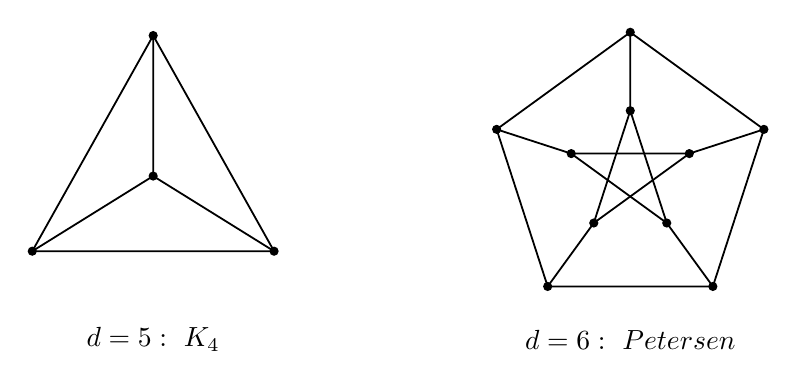
\begin{tikzpicture}[scale=0.83,line width=0.65pt]
\begin{scope}[xshift=-4cm]
\coordinate (a) at (0,2.1);\coordinate (b) at (-1.85,-1.2);
\coordinate (c) at (1.85,-1.2);\coordinate (d) at (0,-0.05);
\draw (a)--(b)--(c)--cycle;
\draw (d)--(a) (d)--(b) (d)--(c);
\foreach \x in {a,b,c,d}{\fill (\x) circle(2pt);}
\node at (0,-2.55) {$d=5:\ K_4$};
\end{scope}
\begin{scope}[xshift=3.3cm]
\foreach \i in {0,...,4}{
\coordinate (A\i) at ({90+72*\i}:2.15);
\coordinate (B\i) at ({90+72*\i}:0.95);}
\foreach \i in {0,...,4}{
\pgfmathtruncatemacro{\j}{mod(\i+1,5)}
\pgfmathtruncatemacro{\k}{mod(\i+2,5)}
\draw (A\i)--(A\j) (A\i)--(B\i) (B\i)--(B\k);
\fill (A\i) circle(2pt);\fill (B\i) circle(2pt);}
\node at (0,-2.55) {$d=6:\ \text{Petersen}$};
\end{scope}
\end{tikzpicture}
\caption{core頂点のlink。右は同時Petersen化した選択の一つ。右図の線分の内部交差はグラフの頂点を表さない。}
\label{fig:links}
\end{figure}

\subsection{通常の閉じたaffine surfaceとの区別}
\begin{corollary}\label{inv:no-almost-toric}
$d\ge5$の$X_d$は、境界のない通常の曲面を基底とし、focus--focus特異点だけを許すclosed almost toric fibrationを持たない。
\end{corollary}
\begin{proof}
Leung--Symingtonの分類\cite[Theorem 2.1, Table 1]{LeungSymington}では、この場合の全空間はK3、Enriques、または対応するtorus bundlesである。
そのEuler数はそれぞれ24、12、0である。
式\eqref{inv:euler}の値は$d\ge5$で55以上なので、いずれとも一致しない。
\end{proof}

定理\ref{main:global}が許すbranchとcoreは、この制約と両立している。
一方、coreの型を次数によらず有限個に制限できるか、分岐を含む底空間にどのtropical構造を与えられるかは、この構成の次に残る問題である。
